
All code was implemented in the Julia language due to the availability of \textit{packages} for subproblems of this work. In the next section, several components of the solution to the problem of optimization of impulsive maneuvers are detailed, along with its full formulation.

\section{Orbit Propagation}

The implementation of an orbit propagator concerns itself with the implementation of the function \(p_o(X, t)\) introduced in equation~\eqref{eq:orbit_propagator}. Two different cases are to be considered: "explicit" propagation, where numerical inputs are available and a numerical output is desired; and "implicit" propagation, where the propagation step is a part of a larger solver.

Brazil's INPE developed a package for orbit propagation and analysis with several models (Kepler, J2 semi-analytical secular and short term, among others) CITE called \texttt{SatelliteToolbox}. It provides quite convient functions for converting between the Cartesian state vector \(\begin{bmatrix}
    r^T & v^T
\end{bmatrix}^T\) and the Keplerian elements, as well as functions for the propagation of orbits by some specified amount of time \(t_p\). Its algorithms take into account all sorts of singularities and edge cases CITE REF OF ANOMALIES, making it numerically precise but unsuitable for nonlinear solvers, which expect differentiable functions everywhere. The functions in this package are also limited to elliptic orbits.

Therefore, this is an auxiliary package used for verification, initial guess generation, and direct numerical propagation whenever required. When propagation is required in the statement of a nonlinear optimization problem, another method for orbit propagation is required. Discretized numerical integration in Cartesian coordinates was chosen for this. Discretized integration inside a numerical solver is done via collocation, a shooting method, or via relaxation. READ ON SINGLE VS MULTIPLE SHOOTING VS RELAXATION

Let \(X_{\text{next}} = f_{RK}(X_{\text{prev}}, \Delta t)\) be the (two-body) dynamics function discretized through a fourth order Runge Kutta method. Then a number \(N\) of integration steps is chosen and \(N+1\) state vector variables \(X_j, j=1,\dots,N+1\) are created. They are subject to the constraints
\begin{equation}
    X_{k+1} = f_{RK}(X_k, \frac{t_p}{N}), k = 1, \dots, N.
\end{equation}
This leaves \(\dim X = 6\) degrees of freedom, which are to be specified with a boundary condition. This boundary condition can be an initial condition, a final condition or relation to another coasting segment through an impulse, as will be discussed in Section~\ref{sec:impulsive_statement}. Thus, this parameterization of orbital propagation is \textit{isoconstrained}.

\section{Nonlinear solver}

Nonlinear solvers are algorithms which iteratively approximate the solution to a system of nonlinear equations or a constrained optimization problem. Many algorithms, and many different algorithms exist. Broadly speaking, there are two classes of algorithms: gradient-free and gradient based. Gradient-free methods do not rely on derivatives for finding a solution; prototypical examples are Simplex methods, evolutionary algorithms, and simulated annealing. They are quite general but do not fully exploit a problem's structure when derivative information is available. Gradient-based methods include gradient descent, sequential quadratic programming (SQP), Newton-Raphson, trust-region methods and interior point methods. A sophisticated implementation of an interior point method is found in Ipopt, an open-source solver with interfaces in many languages CITE.

A further distinction between algorithms is whether they are local or global solvers. Local solvers will converge (usually quickly) to a local optimum, which is not certified to be the global optimum (and in general, should not be assumed to be). Thus they rely on good initial guesses, to be provided to the solver, to arrive at an extremum. Global solvers can discover multiple local extrema and select the best among them; they sometimes rely on multiple (possibly random) initial values for a local optimizer.

Julia offers a multitude of nonlinear solvers, each with different scope, interface, and algorithms. This work has chosen to use \texttt{JuMP}, a package which offers a modelling language for optimization problems that is quite close to mathematical notation. The package's \textit{tech stack} can be seen in figure~\ref{fig:tech_stack}. Internally, \texttt{JuMP} relies on an intermediary package, \texttt{MathOptInterface}, which standardizes solver interfaces. This in turn allows for the usage of \texttt{Ipopt\_jll}, an unofficial wrapper for the Ipopt solver. Ipopt is an open-source nonlinear solver widely recognized for its speed and precision, outperforming many competitors and being quite flexible. It is especially well suited to problems with many variables (up to thousands) with sparse constraints (that is, constraints that depend only on small subsets of variables). It is capable of handling equality and inequality constraints.

This solver allows for the specification of lower and upper bounds of variables separately to the specification of inequality constraints. Variable bounds are guaranteed to be respected at all iterations; inequality constraints are only guaranteed to be satisfied at the converged solution, if the problem is feasible. This distinction is important because some constraints define the domain of problem and should never be violated; other constraints are problem-based and therefore can be violated during the iteration process.

Finally, Ipopt is built with sparsity in mind. Complex calculations should be broken into simpler constraints, each depending on less variables. This may even increase the number of variables but Ipopt's performance profits from this structure.

\begin{figure}[htbp]
    \centering
        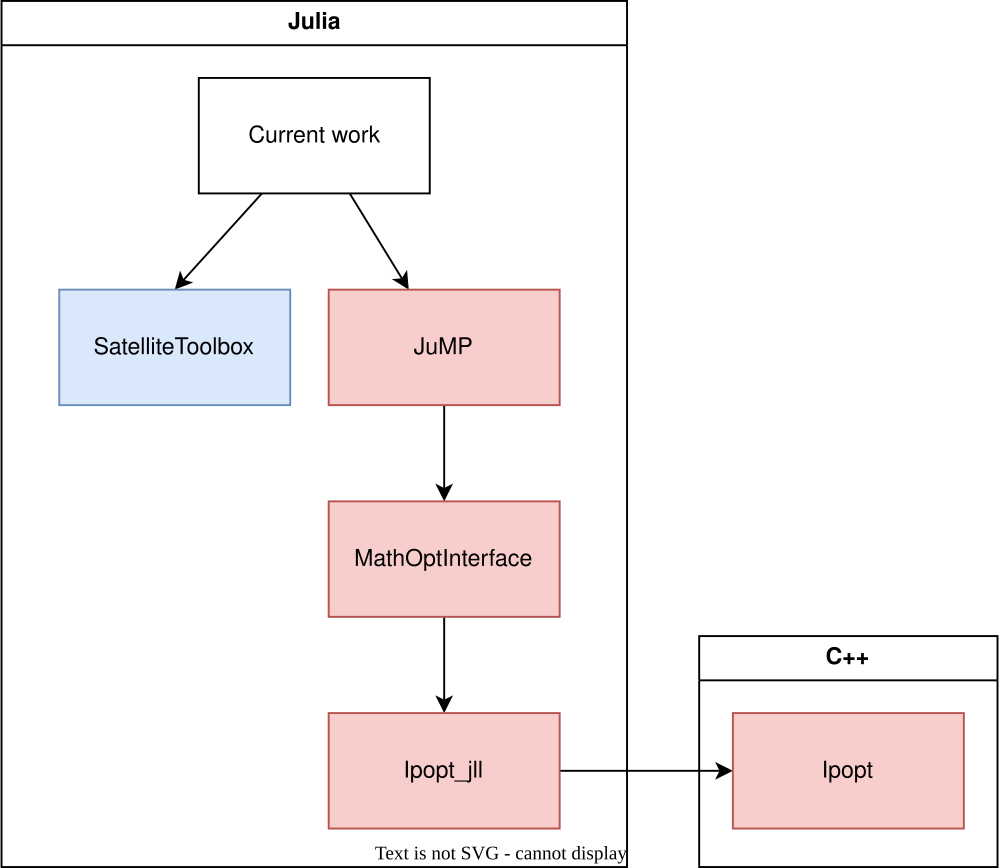
\includegraphics[width=\textwidth]{img/techstack.png}
    \caption{Relationship of code components}
    \label{fig:tech_stack}
\end{figure}

\section{Lambert problem formulations}



\section{Optimal impulsive maneuver problem statement} \label{sec:impulsive_statement}

algo usado